\documentclass{article} 
\usepackage{listings}
\usepackage{graphicx}
\usepackage{subfig}
\usepackage{multirow}

\lstset
{ %Formatting for code in appendix
    language=Python,
    %basicstyle=\footnotesize,
    numbers=left,
    stepnumber=1,
    showstringspaces=true,
    tabsize=4,
    breaklines=true,
    breakatwhitespace=false,
}

\title{AI 534 IA2 Report}
\author{Rishab Balasubramanian}
\date{}

\begin{document}
\maketitle
\textbf{Part1.}a. As we increase lambda, we see from Fig.\ref{fig:L2_vs_lambda} that the training accuracy slowly reduces, while dev accuracy increases slightly. After a point ($\lambda=0.01$), both accuracies start falling. This shows that the accuracy improves upto some regularization parameter $\lambda$ (by reducing overfitting), after which the accuracy decreases (because of underfitting trying to minimize the weights), which can be attributed to the fact that for a larger $\lambda$, we place more importance on minimizing weights, which thus dominate the gradient. Based on the validation accuacry $\lambda=0.001$ gives best results (Validation accuracy = $78.97\%$).\\

\begin{table}[h]
\caption{Largest Parameters from L2 Regularization}
\begin{tabular}{ |p{6cm}||p{6cm}|  }
 \hline
 \multicolumn{2}{|c|}{$\lambda_{-} = 0.0001$} \\
 \hline
 Parameter Name & Weight Value\\
 \hline
Previously$\_$Insured  &     2.212278\\
Vehicle$\_$Damage      &     1.851492\\
Driving$\_$License      &    1.203679\\
Policy$\_$Sales$\_$Channel$\_$78 & 0.983048\\
Policy$\_$Sales$\_$Channel$\_$37 & 0.977445\\
 \hline
 \multicolumn{2}{|c|}{$\lambda_{*} = 0.001$} \\
 \hline
 Parameter Name & Weight Value\\
 \hline
Previously$\_$Insured   &    2.184518\\
Vehicle$\_$Damage        &   1.754571\\
dummy                  &  1.228644\\
Policy$\_$Sales$\_$Channel$\_$20 & 0.894057\\
Policy$\_$Sales$\_$Channel$\_$64  &0.887815\\
\hline
\multicolumn{2}{|c|}{$\lambda_{+} = 0.01$} \\
 \hline
 Parameter Name & Weight Value\\
 \hline
Vehicle$\_$Damage        &    1.580687\\
Previously$\_$Insured     &   1.496561\\
dummy                   &  0.980942\\
Policy$\_$Sales$\_$Channel$\_$26  & 0.454201\\
Policy$\_$Sales$\_$Channel$\_$152 & 0.420518\\
\hline
\end{tabular}
\label{table:L2}
\end{table}
\vspace{\baselineskip}


\begin{figure}[!h]
    \centering
    \subfloat[\centering $\lambda$ = 0.0001]{{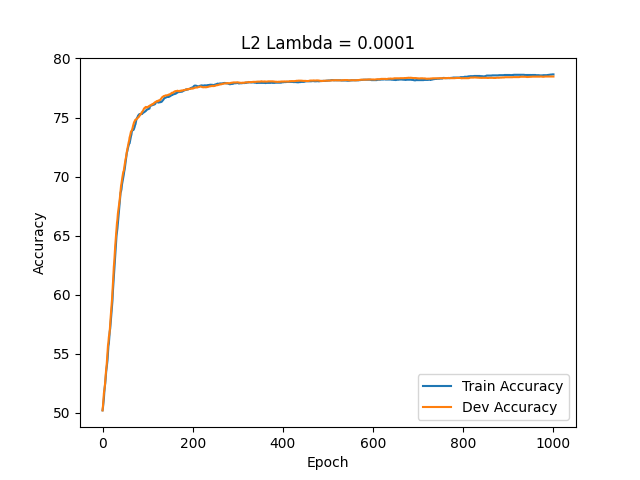
\includegraphics[width=0.32\textwidth, height=4cm]{./figs/L2 lamda = 0.0001.png} }}
    \subfloat[\centering $\lambda$ = 0.001]{{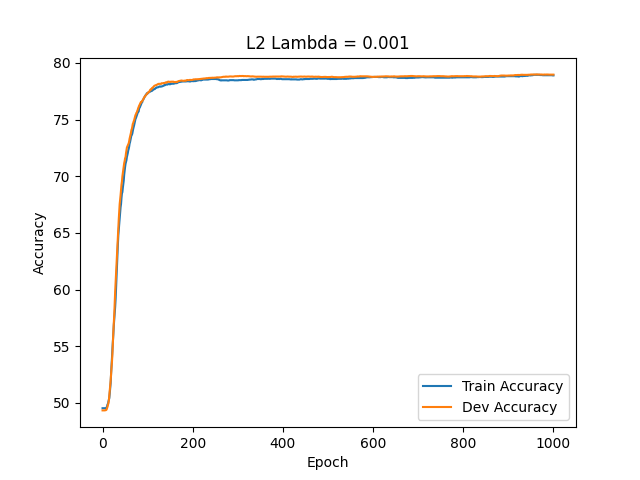
\includegraphics[width=0.32\textwidth, height=4cm]{./figs/L2 lamda = 0.001.png} }}
    \subfloat[\centering $\lambda$ = 0.01]{{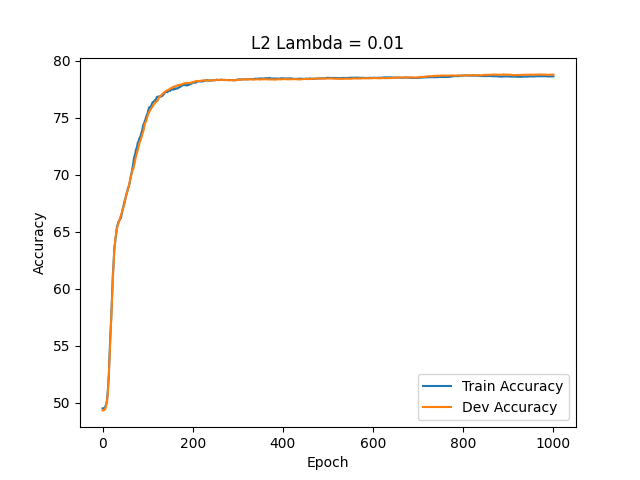
\includegraphics[width=0.32\textwidth, height=4cm]{./figs/L2 lamda = 0.01.png} }}\\
    \subfloat[\centering $\lambda$ = 0.1]{{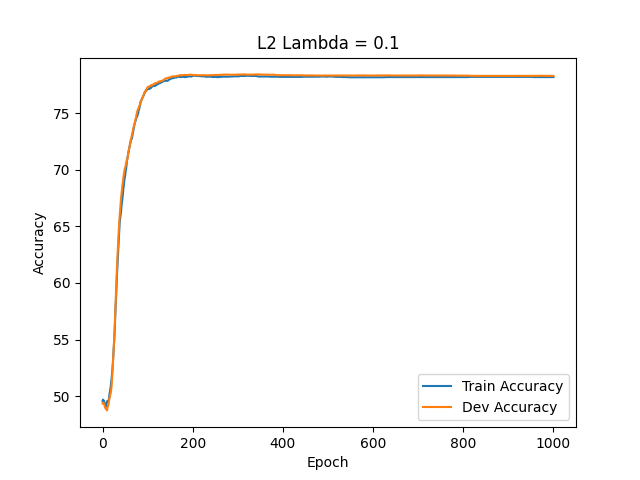
\includegraphics[width=0.32\textwidth, height=4cm]{./figs/L2 lamda = 0.1.png} }}
    \subfloat[\centering $\lambda$ = 1]{{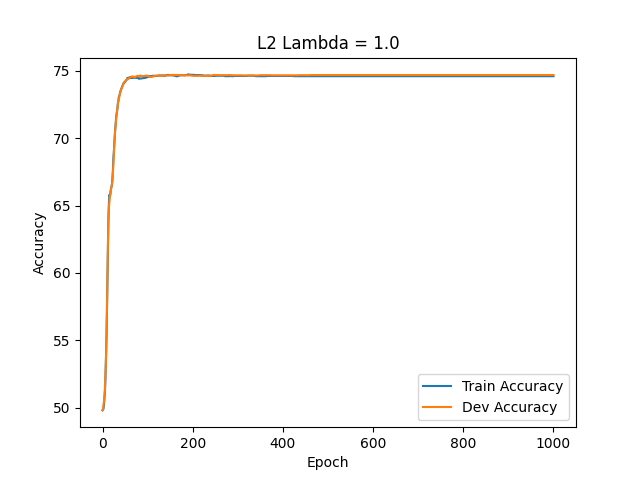
\includegraphics[width=0.32\textwidth, height=4cm]{./figs/L2 lamda = 1.0.png} }}
    \subfloat[\centering $\lambda$ = 10]{{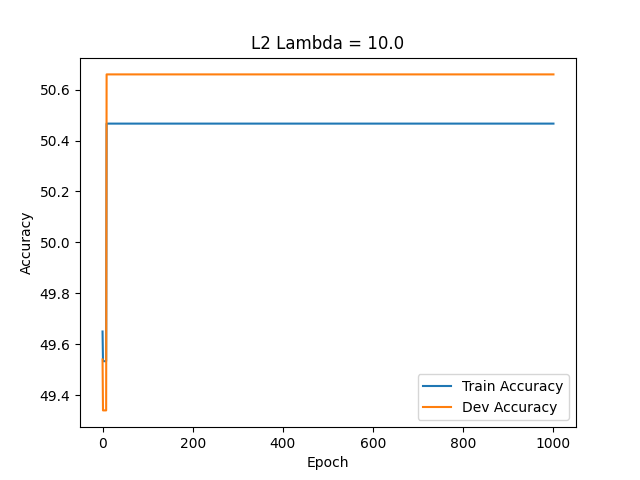
\includegraphics[width=0.32\textwidth, height=4cm]{./figs/L2 lamda = 10.0.png} }}\\
    \subfloat[\centering L2 Accuracy vs $\lambda$]{{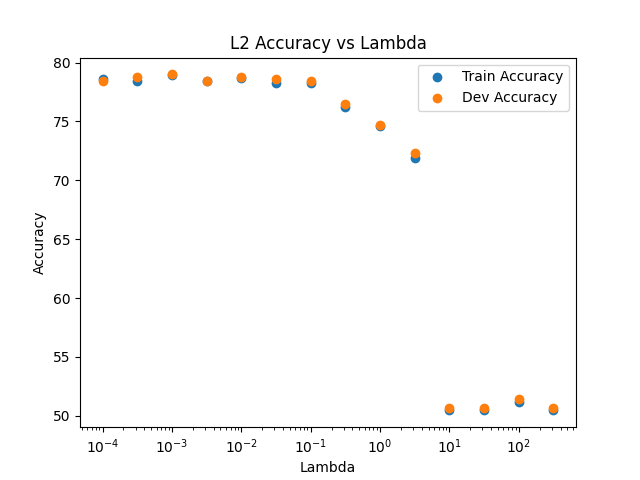
\includegraphics[width=0.75\textwidth, height=6cm]{./figs/L2 Accuracy vs lambda.png} }}\\
\caption{Model Accuracy with L2 regularization}
    \label{fig:L2_vs_lambda}%
\end{figure}

b. We can clearly observe from Table.\ref{table:L2} the magnitude of the weights reduces as we increase the regularization parameter $\lambda$. We see that for $\lambda=0.0001$, the average of the top five largest weights is $1.4455$, for $\lambda=0.001$ it is $1.38988$ and for $\lambda=0.01$ it is $0.98655$. This shows the effect of regularization on reducing the magnitude of weights at higher values of $\lambda$ due to the regularization contributing more to the gradient.\\
\vspace{\baselineskip}

c. Fig.\ref{fig:L2_sparsity} shows the variation of the sparsity of the weights with $\lambda$. We see that for some particular value of $\lambda$, the weights become highly sparse. This turns out to be close to the optimal value of $\lambda$, and thus we can assume these weights to be optimal. However, as we continue to increase $\lambda$, we see that the sparsity reduces again. This shows the property of the L2 regularization which prevents sparse weights. If we further increase $\lambda$, the weights would go close to zero, but all of them will never become $0$ simultaneously. This is attibuted to the gradient of L2 regularization, which is proportional to the value of the weight, and thus the magnitude of the gradient decreases as the magnitude of the weight decreases.

\begin{figure}[!h]
    \centering
    \subfloat[\centering Sparsity for L2 Regularization ($w = 0$)]{{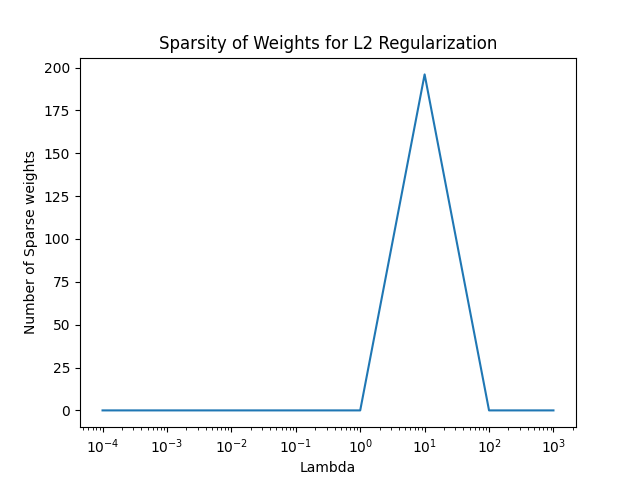
\includegraphics[width=0.75\textwidth, height=6cm]{./figs/L2 sparsity_v2.png} }}
\caption{Number of Sparse weights vs $\lambda$}
    \label{fig:L2_sparsity}
\end{figure}



\textbf{Part 2.} a. We can see from Fig.\ref{fig:L1_vs_lambda} that similar to Part 1, while $\lambda$ increases upto a particular value ($\lambda=0.01$), the validation accuracy increases and training accuraccy reduces showing that the regularization helps prevent overfitting. Beyond this value of $\lambda$, the model begins to underfit. Based on the validation accuracy, $\lambda=0.001$ gives the best accuracy of $78.84\%$. \\

b. We can clearly observe from Table.\ref{table:L1} that, similar to Part 1, the magnitude of the weights reduces as we increase the regularization parameter $\lambda$. We see that for $\lambda=0.0001$, the average of the top five largest weights is $1.4107$, for $\lambda=0.001$ it is $1.37866$ and for $\lambda=0.01$ it is $1.011$. This shows the effect of regularization on reducing the magnitude of weights as $\lambda$ becomes very large, highlighting the underfitting of the model.\\

\begin{table}
\caption{Largest Parameters from L1 Regularization}
\begin{tabular}{ |p{6cm}||p{6cm}|  }
 \hline 
 \multicolumn{2}{|c|}{$\lambda_{-} = 0.0001$} \\
 \hline
 Parameter Name & Weight Value\\
 \hline
Previously$\_$Insured       & 2.105241\\
Vehicle$\_$Damage           & 1.916172\\
Driving$\_$License          & 1.054955\\
Policy$\_$Sales$\_$Channel$\_$132  &0.988875\\
Policy$\_$Sales$\_$Channel$\_$130 & 0.988164\\

 \hline
 \multicolumn{2}{|c|}{$\lambda_{*} = 0.001$} \\
 \hline
 Parameter Name & Weight Value\\
 \hline
Previously$\_$Insured    &    2.224153\\
Vehicle$\_$Damage         &   1.813022\\
dummy                  &   1.087429\\
Policy$\_$Sales$\_$Channel$\_$119&  0.890106\\
Region$\_$Code$\_$51           & 0.878618\\

 
 \hline
\multicolumn{2}{|c|}{$\lambda_{+} = 0.01$} \\
 \hline
 Parameter Name & Weight Value\\
 \hline
Previously$\_$Insured   &     1.825255\\
Vehicle$\_$Damage        &    1.711125\\
dummy                  &   0.988511\\
Policy$\_$Sales$\_$Channel$\_$152&  0.265840\\
Vehicle$\_$Age$\_$1            & 0.265746\\
\hline
\end{tabular}
\label{table:L1}
\end{table}
\vspace{\baselineskip}

c. Fig.\ref{fig:L1_sparsity} shows that as we increase $\lambda$ the number of parameters that become (approximately) $0$ increases almost linearly till all features become sparse. This is different from Part 1, where not all features became sparse, highlighting that L1-regularization makes the weights sparse. This is due to the nature of the gradient of the L1 regularization which is either 1 (when $w > 0$), -1 (when $w<0$) or 0 (when $w=0$). Therefore the weights would be driven to zero (or very close to 0) very quickly, and oscillate there. If we continue to increase $\lambda$, the number of sparse weights increases (if all the weights are not 0 already), or stays constant if all the weights are already sparse.\\

\begin{figure}[!h]
    \centering
    \subfloat[\centering Sparsity for L1 Regularization]{{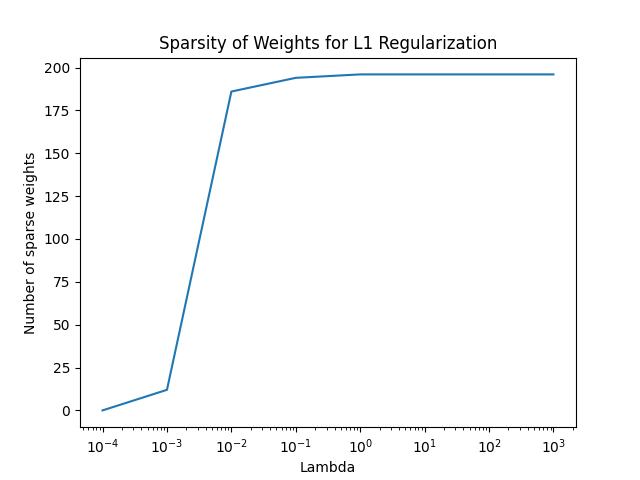
\includegraphics[width=0.75\textwidth, height=6cm]{./figs/L1 sparsity.png} }}\\
\caption{Number of Sparse weights vs $\lambda$}
    \label{fig:L1_sparsity}
\end{figure}


\begin{figure}[h]
    \centering
    \subfloat[\centering $\lambda$ = 0.0001]{{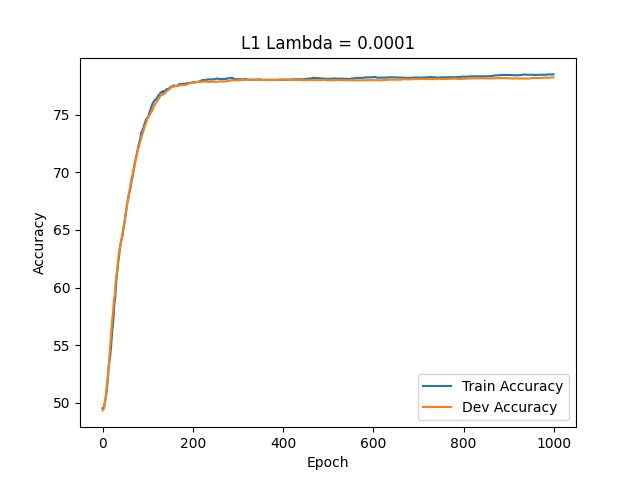
\includegraphics[width=0.32\textwidth, height=4cm]{./figs/L1 lamda = 0.0001.png} }}
    \subfloat[\centering $\lambda$ = 0.001]{{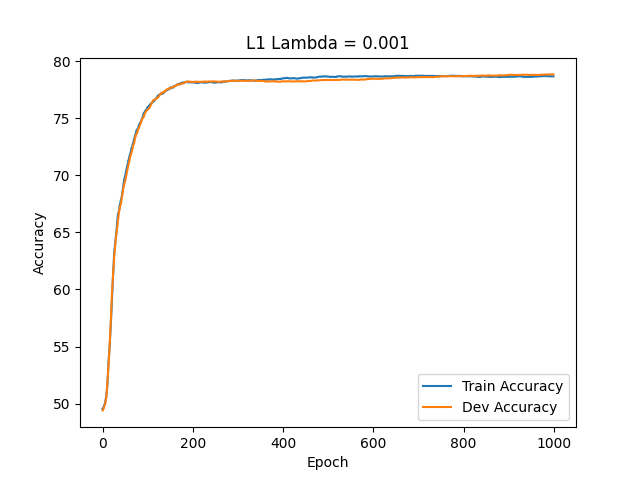
\includegraphics[width=0.32\textwidth, height=4cm]{./figs/L1 lamda = 0.001.png} }}
    \subfloat[\centering $\lambda$ = 0.01]{{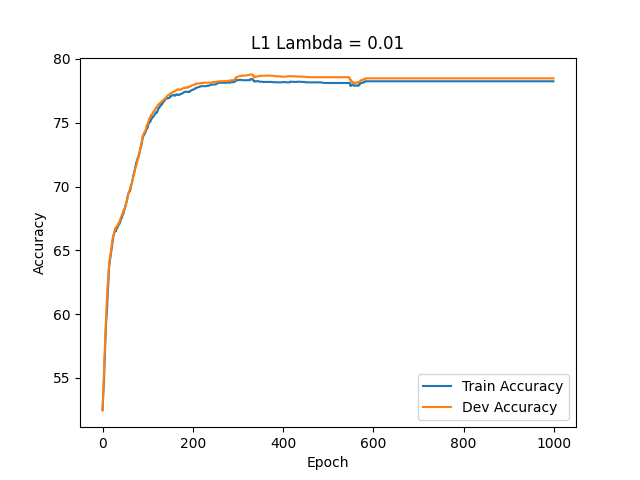
\includegraphics[width=0.32\textwidth, height=4cm]{./figs/L1 lamda = 0.01.png} }}\\
    \subfloat[\centering $\lambda$ = 0.1]{{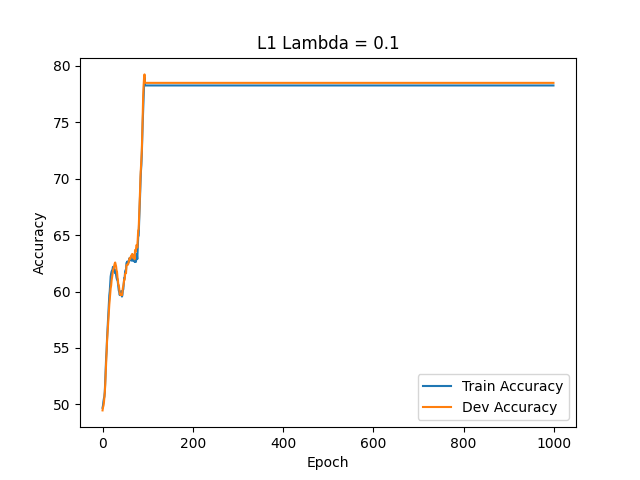
\includegraphics[width=0.32\textwidth, height=4cm]{./figs/L1 lamda = 0.1.png} }}
    \subfloat[\centering $\lambda$ = 1]{{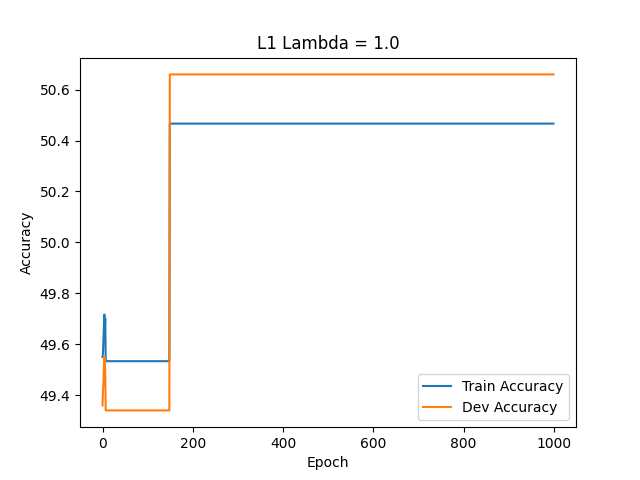
\includegraphics[width=0.32\textwidth, height=4cm]{./figs/L1 lamda = 1.0.png} }}
    \subfloat[\centering $\lambda$ = 10]{{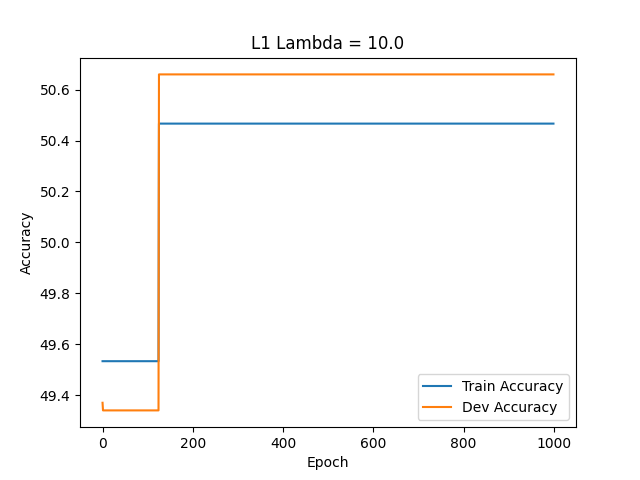
\includegraphics[width=0.32\textwidth, height=4cm]{./figs/L1 lamda = 10.0.png} }}\\
    \subfloat[\centering L1 Accuracy vs $\lambda$]{{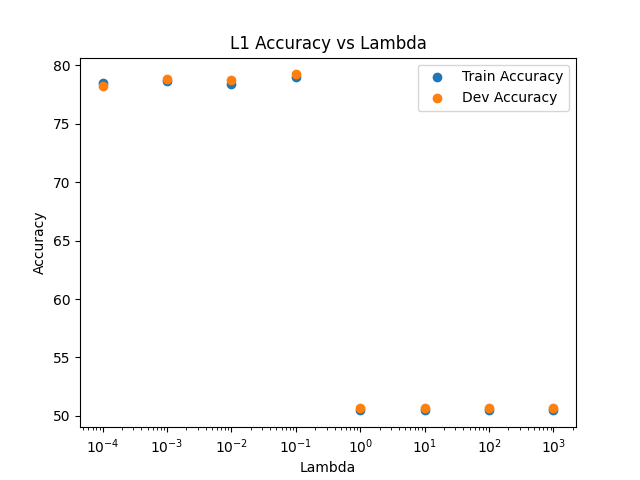
\includegraphics[width=0.75\textwidth, height=6cm]{./figs/L1 Accuracy vs lambda.png} }}\\
\caption{Model Accuracy with L1 regularization}
    \label{fig:L1_vs_lambda}%
\end{figure}

\textbf{Part3.} In this part I tried varying the regularization to check if increasing data would have an impact on the regularization. I found that with more data, a lower regularization worked better. Next I tried to reduce the number of features. I found that the values for Region$\_$Code$\_(j)$ and Policy$\_$Sales$\_$Channel$\_(i)$ were only $1$ for a unique value of $j$ and $i$. That is for a particular customer, amongst the 154 Policy Sales Channels, only one was used, and likewise so for the Region Code. Thus I converted these to single integers, based on which $i$ and $j$ were used for each customer. The new data-model converged to $78.37\%$, which was lower than the original data accuracy. I think that the prediction accuracy is limited by both the data and the model. The data have little correlation, and therefore it is not possible to generate higher dimensional data from the ones provided. But I think the model is the biggest limitation in this framework. Logistic regression provides a linear boundary, which limits the accuracy. Using some other model, which could provide non-linear decision boundaries could improve accuracy.


\end{document}